% Former Figure 1 of the WSDM draft (moved to the repository).
% Needs pgfplots.
\begin{figure*}[t]
\centering
\pgfplotsset{probeplot/.style={width=0.285\textwidth, height=3.3cm,
  xlabel={seconds per query}, xlabel style={font=\footnotesize},
  ticklabel style={font=\scriptsize}, title style={font=\footnotesize},
  ylabel style={font=\footnotesize}, mark size=1.2pt, line width=0.7pt,
  grid=major, grid style={gray!20}}}
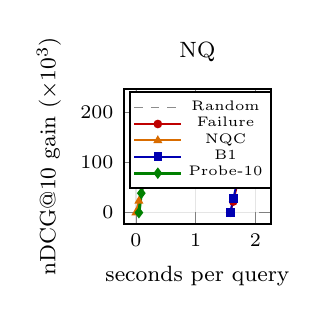
\begin{tikzpicture}
\begin{axis}[probeplot, title={NQ}, ylabel={nDCG@10 gain ($\times10^3$)},
  legend style={font=\tiny, at={(0.52,0.98)}, anchor=north, row sep=-3pt, inner sep=1pt}]
\addplot[black!45, dashed, mark=none] coordinates {(0,0)(0.05,22.5)(0.12,56.3)(0.24,112.5)(0.36,168.8)(0.48,225.1)};
\addplot[red!75!black, mark=*] coordinates {(1.58,0)(1.63,22.1)(1.70,57.6)(1.82,113.5)(1.94,175.1)(2.06,225.1)};
\addplot[orange!85!black, mark=triangle*] coordinates {(0,0)(0.05,23.3)(0.12,52.9)(0.24,107.5)(0.36,162.8)(0.48,225.1)};
\addplot[blue!70!black, mark=square*] coordinates {(1.58,0)(1.63,28.1)(1.70,63.7)(1.82,126.4)(1.94,180.4)(2.06,225.1)};
\addplot[green!50!black, mark=diamond*, line width=1.1pt] coordinates {(0.05,0)(0.09,38.8)(0.15,81.8)(0.25,149.0)(0.36,195.5)(0.46,225.1)};
\legend{Random, Failure, NQC, B1, Probe-10}
\end{axis}
\end{tikzpicture}\hfill
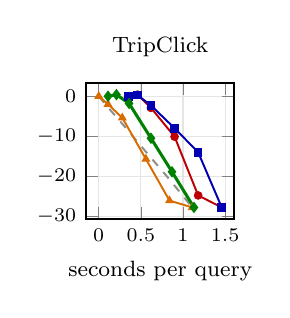
\begin{tikzpicture}
\begin{axis}[probeplot, title={TripClick}]
\addplot[black!45, dashed, mark=none] coordinates {(0,0)(0.11,-2.8)(0.28,-6.9)(0.56,-13.9)(0.84,-20.8)(1.11,-27.8)};
\addplot[red!75!black, mark=*] coordinates {(0.35,0)(0.46,0.4)(0.62,-2.9)(0.90,-10.1)(1.18,-24.8)(1.46,-27.8)};
\addplot[orange!85!black, mark=triangle*] coordinates {(0,0)(0.11,-2.0)(0.28,-5.4)(0.56,-15.7)(0.84,-26.1)(1.11,-27.8)};
\addplot[blue!70!black, mark=square*] coordinates {(0.35,0)(0.46,0.3)(0.62,-2.3)(0.90,-8.0)(1.18,-14.0)(1.46,-27.8)};
\addplot[green!50!black, mark=diamond*, line width=1.1pt] coordinates {(0.11,0)(0.21,0.4)(0.36,-1.8)(0.62,-10.5)(0.87,-18.9)(1.13,-27.8)};
\end{axis}
\end{tikzpicture}\hfill
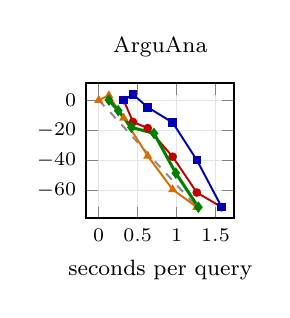
\begin{tikzpicture}
\begin{axis}[probeplot, title={ArguAna}]
\addplot[black!45, dashed, mark=none] coordinates {(0,0)(0.13,-7.1)(0.32,-17.8)(0.63,-35.6)(0.95,-53.4)(1.26,-71.1)};
\addplot[red!75!black, mark=*] coordinates {(0.32,0)(0.44,-14.5)(0.63,-18.6)(0.95,-37.6)(1.26,-61.4)(1.58,-71.1)};
\addplot[orange!85!black, mark=triangle*] coordinates {(0,0)(0.13,3.1)(0.32,-11.8)(0.63,-37.1)(0.95,-59.4)(1.26,-71.1)};
\addplot[blue!70!black, mark=square*] coordinates {(0.32,0)(0.44,3.8)(0.63,-4.8)(0.95,-14.9)(1.26,-39.8)(1.58,-71.1)};
\addplot[green!50!black, mark=diamond*, line width=1.1pt] coordinates {(0.13,0)(0.25,-7.0)(0.42,-18.1)(0.71,-22.1)(0.99,-48.5)(1.28,-71.1)};
\end{axis}
\end{tikzpicture}\hfill
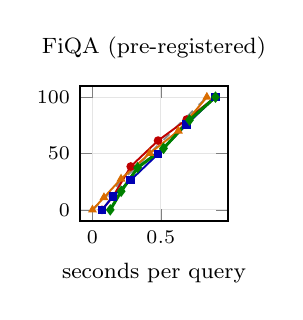
\begin{tikzpicture}
\begin{axis}[probeplot, title={FiQA (pre-registered)}]
\addplot[black!45, dashed, mark=none] coordinates {(0,0)(0.084,10.0)(0.209,25.0)(0.419,50.1)(0.628,75.1)(0.837,100.1)};
\addplot[red!75!black, mark=*] coordinates {(0.07,0)(0.15,11.8)(0.28,38.5)(0.48,61.5)(0.69,80.2)(0.90,100.1)};
\addplot[orange!85!black, mark=triangle*] coordinates {(0,0)(0.084,11.0)(0.209,27.5)(0.419,50.2)(0.628,70.1)(0.837,100.1)};
\addplot[blue!70!black, mark=square*] coordinates {(0.07,0)(0.15,12.1)(0.28,26.4)(0.48,49.7)(0.69,76.0)(0.90,100.1)};
\addplot[green!50!black, mark=diamond*, line width=1.1pt] coordinates {(0.13,0)(0.21,16.5)(0.33,37.4)(0.52,54.6)(0.71,79.7)(0.90,100.1)};
\end{axis}
\end{tikzpicture}
\caption{Reranking gain over BM25 against measured cost per query
(exploratory) at $0$--$100\%$ of queries reranked; cost is telemetry
(Failure, B1, paid before deciding; on FiQA it includes BM25 retrieval)
or the probe, plus reranking. Oracle (off scale): $0.25$, $0.06$,
$0.10$, $0.12$.}
\label{fig:probe}
\end{figure*}
